\documentclass[twoside]{book}

% Packages required by doxygen
\usepackage{fixltx2e}
\usepackage{calc}
\usepackage{doxygen}
\usepackage[export]{adjustbox} % also loads graphicx
\usepackage{graphicx}
\usepackage[utf8]{inputenc}
\usepackage{makeidx}
\usepackage{multicol}
\usepackage{multirow}
\PassOptionsToPackage{warn}{textcomp}
\usepackage{textcomp}
\usepackage[nointegrals]{wasysym}
\usepackage[table]{xcolor}

% Font selection
\usepackage[T1]{fontenc}
\usepackage[scaled=.90]{helvet}
\usepackage{courier}
\usepackage{amssymb}
\usepackage{sectsty}
\renewcommand{\familydefault}{\sfdefault}
\allsectionsfont{%
  \fontseries{bc}\selectfont%
  \color{darkgray}%
}
\renewcommand{\DoxyLabelFont}{%
  \fontseries{bc}\selectfont%
  \color{darkgray}%
}
\newcommand{\+}{\discretionary{\mbox{\scriptsize$\hookleftarrow$}}{}{}}

% Page & text layout
\usepackage{geometry}
\geometry{%
  a4paper,%
  top=2.5cm,%
  bottom=2.5cm,%
  left=2.5cm,%
  right=2.5cm%
}
\tolerance=750
\hfuzz=15pt
\hbadness=750
\setlength{\emergencystretch}{15pt}
\setlength{\parindent}{0cm}
\setlength{\parskip}{3ex plus 2ex minus 2ex}
\makeatletter
\renewcommand{\paragraph}{%
  \@startsection{paragraph}{4}{0ex}{-1.0ex}{1.0ex}{%
    \normalfont\normalsize\bfseries\SS@parafont%
  }%
}
\renewcommand{\subparagraph}{%
  \@startsection{subparagraph}{5}{0ex}{-1.0ex}{1.0ex}{%
    \normalfont\normalsize\bfseries\SS@subparafont%
  }%
}
\makeatother

% Headers & footers
\usepackage{fancyhdr}
\pagestyle{fancyplain}
\fancyhead[LE]{\fancyplain{}{\bfseries\thepage}}
\fancyhead[CE]{\fancyplain{}{}}
\fancyhead[RE]{\fancyplain{}{\bfseries\leftmark}}
\fancyhead[LO]{\fancyplain{}{\bfseries\rightmark}}
\fancyhead[CO]{\fancyplain{}{}}
\fancyhead[RO]{\fancyplain{}{\bfseries\thepage}}
\fancyfoot[LE]{\fancyplain{}{}}
\fancyfoot[CE]{\fancyplain{}{}}
\fancyfoot[RE]{\fancyplain{}{\bfseries\scriptsize Generated by Doxygen }}
\fancyfoot[LO]{\fancyplain{}{\bfseries\scriptsize Generated by Doxygen }}
\fancyfoot[CO]{\fancyplain{}{}}
\fancyfoot[RO]{\fancyplain{}{}}
\renewcommand{\footrulewidth}{0.4pt}
\renewcommand{\chaptermark}[1]{%
  \markboth{#1}{}%
}
\renewcommand{\sectionmark}[1]{%
  \markright{\thesection\ #1}%
}

% Indices & bibliography
\usepackage{natbib}
\usepackage[titles]{tocloft}
\setcounter{tocdepth}{3}
\setcounter{secnumdepth}{5}
\makeindex

% Custom commands
\newcommand{\clearemptydoublepage}{%
  \newpage{\pagestyle{empty}\cleardoublepage}%
}

\usepackage{caption}
\captionsetup{labelsep=space,justification=centering,font={bf},singlelinecheck=off,skip=4pt,position=top}

%===== C O N T E N T S =====

\begin{document}

% Titlepage & ToC
\pagenumbering{roman}
\begin{titlepage}
\vspace*{7cm}
\begin{center}%
{\Large Práctica 4 }\\
\vspace*{1cm}
{\large Generated by Doxygen 1.8.11}\\
\end{center}
\end{titlepage}
\clearemptydoublepage
\tableofcontents
\clearemptydoublepage
\pagenumbering{arabic}

%--- Begin generated contents ---
\chapter{Hierarchical Index}
\section{Class Hierarchy}
This inheritance list is sorted roughly, but not completely, alphabetically\+:\begin{DoxyCompactList}
\item \contentsline{section}{Client}{\pageref{class_client}}{}
\item Remote\begin{DoxyCompactList}
\item \contentsline{section}{Client\+\_\+\+Server}{\pageref{interface_client___server}}{}
\begin{DoxyCompactList}
\item \contentsline{section}{Server}{\pageref{class_server}}{}
\end{DoxyCompactList}
\end{DoxyCompactList}
\end{DoxyCompactList}

\chapter{Class Index}
\section{Class List}
Here are the classes, structs, unions and interfaces with brief descriptions\+:\begin{DoxyCompactList}
\item\contentsline{section}{{\bf main} }{\pageref{classmain}}{}
\item\contentsline{section}{{\bf Matrix} \\*\doxyref{Matrix}{p.}{class_matrix} class to create and control a integer matrix.  public }{\pageref{class_matrix}}{}
\end{DoxyCompactList}

\chapter{File Index}
\section{File List}
Here is a list of all files with brief descriptions\+:\begin{DoxyCompactList}
\item\contentsline{section}{C\+:/\+Users/\+Alfredo/workspace/\+P\+\_\+3/src/{\bf A.\+java} }{\pageref{_a_8java}}{}
\item\contentsline{section}{C\+:/\+Users/\+Alfredo/workspace/\+P\+\_\+3/src/{\bf B.\+java} }{\pageref{_b_8java}}{}
\item\contentsline{section}{C\+:/\+Users/\+Alfredo/workspace/\+P\+\_\+3/src/{\bf Contador.\+java} }{\pageref{_contador_8java}}{}
\item\contentsline{section}{C\+:/\+Users/\+Alfredo/workspace/\+P\+\_\+3/src/{\bf main.\+java} }{\pageref{main_8java}}{}
\end{DoxyCompactList}

\chapter{Class Documentation}
\section{arbitro Class Reference}
\label{classarbitro}\index{arbitro@{arbitro}}


creates the main thread with the role of arbiter, is the thread that starts and ends the game is created.  public  


\subsection*{Static Public Member Functions}
\begin{DoxyCompactItemize}
\item 
static void {\bf wait\+Until\+Finished} (Array\+List$<$ Thread $>$ my\+Threads)
\begin{DoxyCompactList}\small\item\em Method wait\+Until\+Finished.\+Wait until they stop running the threads, and then deletes. \end{DoxyCompactList}\item 
static void {\bf start\+Game} ({\bf Pelota} p)
\begin{DoxyCompactList}\small\item\em Method start\+Game, serves to start the game. \end{DoxyCompactList}\item 
static void {\bf stop\+Game} ({\bf Pelota} p)
\begin{DoxyCompactList}\small\item\em Method stop\+Game, serves to stop the game. \end{DoxyCompactList}\item 
static boolean {\bf game\+On} ()
\begin{DoxyCompactList}\small\item\em Method \doxyref{game\+On()}{p.}{classarbitro_a8766f82969f93d67bca1ff438b360002}, used to know if the game is on. \end{DoxyCompactList}\item 
static void {\bf turnos} ({\bf Ping} players[$\,$], int amount, int times)
\begin{DoxyCompactList}\small\item\em Method turnos, serves to assign the turns of the players. \end{DoxyCompactList}\item 
static void {\bf time} (Long stop, {\bf Ping} players[$\,$], int amount)
\begin{DoxyCompactList}\small\item\em Method time, measures the runtime of the game. \end{DoxyCompactList}\item 
static void {\bf option1} (int amount, int execution)  throws Interrupted\+Exception
\begin{DoxyCompactList}\small\item\em Method option1, starting all threat after creating the players and waits. \end{DoxyCompactList}\item 
static void {\bf option2} (int amount, int execution)
\begin{DoxyCompactList}\small\item\em Method option2, playing for amount of time. \end{DoxyCompactList}\item 
static void {\bf main} (String[$\,$] args)  throws Interrupted\+Exception 
\begin{DoxyCompactList}\small\item\em Method Main of the project, where other programs are initialized. \end{DoxyCompactList}\end{DoxyCompactItemize}


\subsection{Detailed Description}
creates the main thread with the role of arbiter, is the thread that starts and ends the game is created.  public 

\subsection{Member Function Documentation}
\index{arbitro@{arbitro}!game\+On@{game\+On}}
\index{game\+On@{game\+On}!arbitro@{arbitro}}
\subsubsection[{game\+On()}]{\setlength{\rightskip}{0pt plus 5cm}static boolean arbitro.\+game\+On (
\begin{DoxyParamCaption}
{}
\end{DoxyParamCaption}
)\hspace{0.3cm}{\ttfamily [static]}}\label{classarbitro_a8766f82969f93d67bca1ff438b360002}


Method \doxyref{game\+On()}{p.}{classarbitro_a8766f82969f93d67bca1ff438b360002}, used to know if the game is on. 

\begin{DoxyReturn}{Returns}
void  public 
\end{DoxyReturn}
\index{arbitro@{arbitro}!main@{main}}
\index{main@{main}!arbitro@{arbitro}}
\subsubsection[{main(\+String[] args)}]{\setlength{\rightskip}{0pt plus 5cm}static void arbitro.\+main (
\begin{DoxyParamCaption}
\item[{String[$\,$]}]{args}
\end{DoxyParamCaption}
) throws Interrupted\+Exception\hspace{0.3cm}{\ttfamily [static]}}\label{classarbitro_a5815f5b2de4cf471ff518e499aafc9c6}


Method Main of the project, where other programs are initialized. 


\begin{DoxyParams}{Parameters}
{\em args} & \\
\hline
\end{DoxyParams}
\begin{DoxyReturn}{Returns}
void 
\end{DoxyReturn}

\begin{DoxyExceptions}{Exceptions}
{\em Interrupted\+Exception} & public static \\
\hline
\end{DoxyExceptions}
\index{arbitro@{arbitro}!option1@{option1}}
\index{option1@{option1}!arbitro@{arbitro}}
\subsubsection[{option1(int amount, int execution)}]{\setlength{\rightskip}{0pt plus 5cm}static void arbitro.\+option1 (
\begin{DoxyParamCaption}
\item[{int}]{amount, }
\item[{int}]{execution}
\end{DoxyParamCaption}
) throws Interrupted\+Exception\hspace{0.3cm}{\ttfamily [static]}}\label{classarbitro_a834886a9e64c73269fcb27c5e91d2465}


Method option1, starting all threat after creating the players and waits. 


\begin{DoxyParams}{Parameters}
{\em integer} & amount, integer execution \\
\hline
\end{DoxyParams}
\begin{DoxyReturn}{Returns}
void 
\end{DoxyReturn}

\begin{DoxyExceptions}{Exceptions}
{\em Interrupted\+Exception} & public static \\
\hline
\end{DoxyExceptions}
\index{arbitro@{arbitro}!option2@{option2}}
\index{option2@{option2}!arbitro@{arbitro}}
\subsubsection[{option2(int amount, int execution)}]{\setlength{\rightskip}{0pt plus 5cm}static void arbitro.\+option2 (
\begin{DoxyParamCaption}
\item[{int}]{amount, }
\item[{int}]{execution}
\end{DoxyParamCaption}
)\hspace{0.3cm}{\ttfamily [static]}}\label{classarbitro_a68c57a3457bca90c744b32983d1262af}


Method option2, playing for amount of time. 


\begin{DoxyParams}{Parameters}
{\em integer} & amount, integer execution \\
\hline
\end{DoxyParams}
\begin{DoxyReturn}{Returns}
void  public static 
\end{DoxyReturn}
\index{arbitro@{arbitro}!start\+Game@{start\+Game}}
\index{start\+Game@{start\+Game}!arbitro@{arbitro}}
\subsubsection[{start\+Game(\+Pelota p)}]{\setlength{\rightskip}{0pt plus 5cm}static void arbitro.\+start\+Game (
\begin{DoxyParamCaption}
\item[{{\bf Pelota}}]{p}
\end{DoxyParamCaption}
)\hspace{0.3cm}{\ttfamily [static]}}\label{classarbitro_a1100d8415902340de1297abcf6a5560e}


Method start\+Game, serves to start the game. 


\begin{DoxyParams}{Parameters}
{\em \doxyref{Pelota}{p.}{class_pelota}} & p \\
\hline
\end{DoxyParams}
\begin{DoxyReturn}{Returns}
void  public 
\end{DoxyReturn}
\index{arbitro@{arbitro}!stop\+Game@{stop\+Game}}
\index{stop\+Game@{stop\+Game}!arbitro@{arbitro}}
\subsubsection[{stop\+Game(\+Pelota p)}]{\setlength{\rightskip}{0pt plus 5cm}static void arbitro.\+stop\+Game (
\begin{DoxyParamCaption}
\item[{{\bf Pelota}}]{p}
\end{DoxyParamCaption}
)\hspace{0.3cm}{\ttfamily [static]}}\label{classarbitro_aeaa7832cb51e604df61fff360758d0ad}


Method stop\+Game, serves to stop the game. 


\begin{DoxyParams}{Parameters}
{\em \doxyref{Pelota}{p.}{class_pelota}} & p \\
\hline
\end{DoxyParams}
\begin{DoxyReturn}{Returns}
void  public 
\end{DoxyReturn}
\index{arbitro@{arbitro}!time@{time}}
\index{time@{time}!arbitro@{arbitro}}
\subsubsection[{time(\+Long stop, Ping players[], int amount)}]{\setlength{\rightskip}{0pt plus 5cm}static void arbitro.\+time (
\begin{DoxyParamCaption}
\item[{Long}]{stop, }
\item[{{\bf Ping}}]{players[$\,$], }
\item[{int}]{amount}
\end{DoxyParamCaption}
)\hspace{0.3cm}{\ttfamily [static]}}\label{classarbitro_a848800fc167b2061e10bd611a38da0de}


Method time, measures the runtime of the game. 


\begin{DoxyParams}{Parameters}
{\em Long} & stop,\doxyref{Ping}{p.}{class_ping} players[],integer amount \\
\hline
\end{DoxyParams}
\begin{DoxyReturn}{Returns}
void  public static 
\end{DoxyReturn}
\index{arbitro@{arbitro}!turnos@{turnos}}
\index{turnos@{turnos}!arbitro@{arbitro}}
\subsubsection[{turnos(\+Ping players[], int amount, int times)}]{\setlength{\rightskip}{0pt plus 5cm}static void arbitro.\+turnos (
\begin{DoxyParamCaption}
\item[{{\bf Ping}}]{players[$\,$], }
\item[{int}]{amount, }
\item[{int}]{times}
\end{DoxyParamCaption}
)\hspace{0.3cm}{\ttfamily [static]}}\label{classarbitro_af2debb6af02609725fa7541b20b8c311}


Method turnos, serves to assign the turns of the players. 


\begin{DoxyParams}{Parameters}
{\em \doxyref{Ping}{p.}{class_ping}} & players[], integer amount, integer times \\
\hline
\end{DoxyParams}
\begin{DoxyReturn}{Returns}
void  public static 
\end{DoxyReturn}
\index{arbitro@{arbitro}!wait\+Until\+Finished@{wait\+Until\+Finished}}
\index{wait\+Until\+Finished@{wait\+Until\+Finished}!arbitro@{arbitro}}
\subsubsection[{wait\+Until\+Finished(\+Array\+List$<$ Thread $>$ my\+Threads)}]{\setlength{\rightskip}{0pt plus 5cm}static void arbitro.\+wait\+Until\+Finished (
\begin{DoxyParamCaption}
\item[{Array\+List$<$ Thread $>$}]{my\+Threads}
\end{DoxyParamCaption}
)\hspace{0.3cm}{\ttfamily [static]}}\label{classarbitro_a8ad0c101b8ea8b6b422bfa17b4e975ca}


Method wait\+Until\+Finished.\+Wait until they stop running the threads, and then deletes. 


\begin{DoxyParams}{Parameters}
{\em Array\+List$<$\+Thread$>$} & my\+Threads \\
\hline
\end{DoxyParams}
\begin{DoxyReturn}{Returns}
void  private 
\end{DoxyReturn}


The documentation for this class was generated from the following file\+:\begin{DoxyCompactItemize}
\item 
C\+:/\+Users/\+Alfredo/workspace/\+P4/src/{\bf arbitro.\+java}\end{DoxyCompactItemize}

\section{Pelota Class Reference}
\label{class_pelota}\index{Pelota@{Pelota}}


creates objects that ball, so that every player knows when he has to play, it will be when the ball is in their possession  public  


\subsection*{Public Member Functions}
\begin{DoxyCompactItemize}
\item 
void {\bf golpear} ({\bf Ping} p)
\begin{DoxyCompactList}\small\item\em Method golpear, serves for a player hits the ball for the other player. \end{DoxyCompactList}\end{DoxyCompactItemize}


\subsection{Detailed Description}
creates objects that ball, so that every player knows when he has to play, it will be when the ball is in their possession  public 

\subsection{Member Function Documentation}
\index{Pelota@{Pelota}!golpear@{golpear}}
\index{golpear@{golpear}!Pelota@{Pelota}}
\subsubsection[{golpear(\+Ping p)}]{\setlength{\rightskip}{0pt plus 5cm}void Pelota.\+golpear (
\begin{DoxyParamCaption}
\item[{{\bf Ping}}]{p}
\end{DoxyParamCaption}
)}\label{class_pelota_a3c93a8d8431530dd99b81d9811e595ce}


Method golpear, serves for a player hits the ball for the other player. 


\begin{DoxyParams}{Parameters}
{\em \doxyref{Ping}{p.}{class_ping}} & p \\
\hline
\end{DoxyParams}
\begin{DoxyReturn}{Returns}
void  public 
\end{DoxyReturn}


The documentation for this class was generated from the following file\+:\begin{DoxyCompactItemize}
\item 
C\+:/\+Users/\+Alfredo/workspace/\+P4/src/{\bf Pelota.\+java}\end{DoxyCompactItemize}

\section{Ping Class Reference}
\label{class_ping}\index{Ping@{Ping}}


It serves to create game players  public.  


Inheritance diagram for Ping\+:\begin{figure}[H]
\begin{center}
\leavevmode
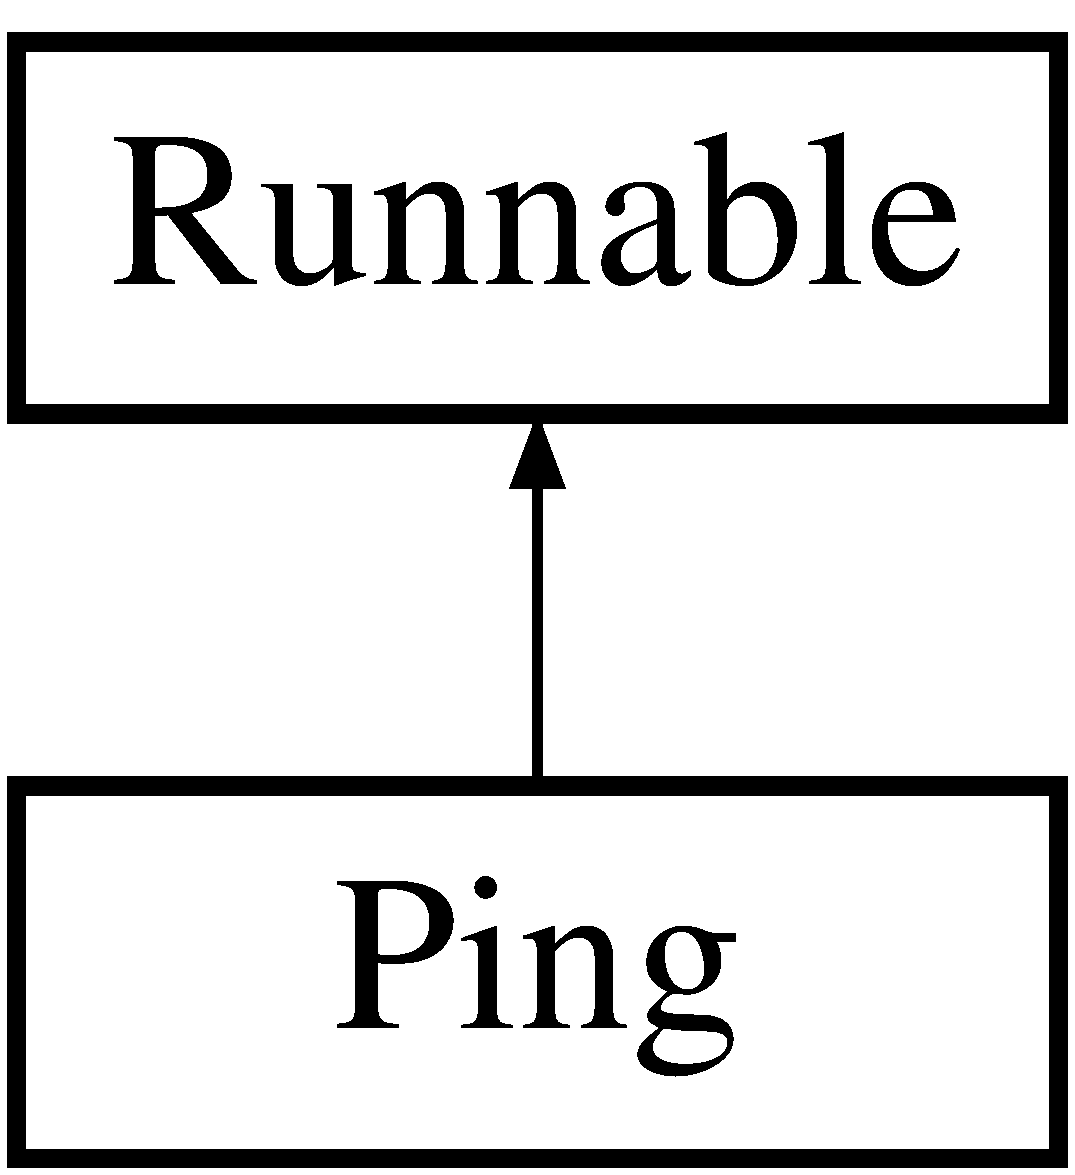
\includegraphics[height=2.000000cm]{class_ping}
\end{center}
\end{figure}
\subsection*{Public Member Functions}
\begin{DoxyCompactItemize}
\item 
{\bf Ping} (String n, {\bf Pelota} p)
\begin{DoxyCompactList}\small\item\em \doxyref{Ping}{p.}{class_ping} constructor, serves to create game players \doxyref{Ping}{p.}{class_ping}. \end{DoxyCompactList}\item 
String {\bf get\+Nombre} ()
\begin{DoxyCompactList}\small\item\em Method \doxyref{get\+Nombre()}{p.}{class_ping_ae3b2b2484ed043ecd02257a62950ae4e}, return the name of the player. \end{DoxyCompactList}\item 
void {\bf set\+Pelota} ()
\begin{DoxyCompactList}\small\item\em Method \doxyref{set\+Pelota()}{p.}{class_ping_af7e942511ee512016bfaaac968c5917b}, serves to give the ball to a player. \end{DoxyCompactList}\item 
void {\bf take\+Ball} ()
\begin{DoxyCompactList}\small\item\em Method \doxyref{take\+Ball()}{p.}{class_ping_a2164defceec530b448193f0db34a0697}, serves to remove the ball to the player. \end{DoxyCompactList}\item 
boolean {\bf has\+It} ()
\begin{DoxyCompactList}\small\item\em Method \doxyref{has\+It()}{p.}{class_ping_ad248ea492a4a04795b21a68f920bc0ee}, used to know if the player has the ball. \end{DoxyCompactList}\item 
void {\bf run} ()
\begin{DoxyCompactList}\small\item\em Run function. Running to start the player \doxyref{Ping}{p.}{class_ping}. \end{DoxyCompactList}\end{DoxyCompactItemize}


\subsection{Detailed Description}
It serves to create game players  public. 

\subsection{Constructor \& Destructor Documentation}
\index{Ping@{Ping}!Ping@{Ping}}
\index{Ping@{Ping}!Ping@{Ping}}
\subsubsection[{Ping(\+String n, Pelota p)}]{\setlength{\rightskip}{0pt plus 5cm}Ping.\+Ping (
\begin{DoxyParamCaption}
\item[{String}]{n, }
\item[{{\bf Pelota}}]{p}
\end{DoxyParamCaption}
)}\label{class_ping_a63e35512f2e5fd005e39985026913854}


\doxyref{Ping}{p.}{class_ping} constructor, serves to create game players \doxyref{Ping}{p.}{class_ping}. 


\begin{DoxyParams}{Parameters}
{\em String} & n, \doxyref{Pelota}{p.}{class_pelota} p  public \\
\hline
\end{DoxyParams}


\subsection{Member Function Documentation}
\index{Ping@{Ping}!get\+Nombre@{get\+Nombre}}
\index{get\+Nombre@{get\+Nombre}!Ping@{Ping}}
\subsubsection[{get\+Nombre()}]{\setlength{\rightskip}{0pt plus 5cm}String Ping.\+get\+Nombre (
\begin{DoxyParamCaption}
{}
\end{DoxyParamCaption}
)}\label{class_ping_ae3b2b2484ed043ecd02257a62950ae4e}


Method \doxyref{get\+Nombre()}{p.}{class_ping_ae3b2b2484ed043ecd02257a62950ae4e}, return the name of the player. 

\begin{DoxyReturn}{Returns}
String  public 
\end{DoxyReturn}
\index{Ping@{Ping}!has\+It@{has\+It}}
\index{has\+It@{has\+It}!Ping@{Ping}}
\subsubsection[{has\+It()}]{\setlength{\rightskip}{0pt plus 5cm}boolean Ping.\+has\+It (
\begin{DoxyParamCaption}
{}
\end{DoxyParamCaption}
)}\label{class_ping_ad248ea492a4a04795b21a68f920bc0ee}


Method \doxyref{has\+It()}{p.}{class_ping_ad248ea492a4a04795b21a68f920bc0ee}, used to know if the player has the ball. 

\begin{DoxyReturn}{Returns}
boolean  public 
\end{DoxyReturn}
\index{Ping@{Ping}!run@{run}}
\index{run@{run}!Ping@{Ping}}
\subsubsection[{run()}]{\setlength{\rightskip}{0pt plus 5cm}void Ping.\+run (
\begin{DoxyParamCaption}
{}
\end{DoxyParamCaption}
)}\label{class_ping_ad8528b6dfdff62253861d4881ecd2c43}


Run function. Running to start the player \doxyref{Ping}{p.}{class_ping}. 

\begin{DoxyReturn}{Returns}
void  public 
\end{DoxyReturn}
\index{Ping@{Ping}!set\+Pelota@{set\+Pelota}}
\index{set\+Pelota@{set\+Pelota}!Ping@{Ping}}
\subsubsection[{set\+Pelota()}]{\setlength{\rightskip}{0pt plus 5cm}void Ping.\+set\+Pelota (
\begin{DoxyParamCaption}
{}
\end{DoxyParamCaption}
)}\label{class_ping_af7e942511ee512016bfaaac968c5917b}


Method \doxyref{set\+Pelota()}{p.}{class_ping_af7e942511ee512016bfaaac968c5917b}, serves to give the ball to a player. 

\begin{DoxyReturn}{Returns}
void  public 
\end{DoxyReturn}
\index{Ping@{Ping}!take\+Ball@{take\+Ball}}
\index{take\+Ball@{take\+Ball}!Ping@{Ping}}
\subsubsection[{take\+Ball()}]{\setlength{\rightskip}{0pt plus 5cm}void Ping.\+take\+Ball (
\begin{DoxyParamCaption}
{}
\end{DoxyParamCaption}
)}\label{class_ping_a2164defceec530b448193f0db34a0697}


Method \doxyref{take\+Ball()}{p.}{class_ping_a2164defceec530b448193f0db34a0697}, serves to remove the ball to the player. 

\begin{DoxyReturn}{Returns}
void  public 
\end{DoxyReturn}


The documentation for this class was generated from the following file\+:\begin{DoxyCompactItemize}
\item 
C\+:/\+Users/\+Alfredo/workspace/\+P4/src/{\bf Ping.\+java}\end{DoxyCompactItemize}

\chapter{File Documentation}
\section{C\+:/\+Users/\+Alfredo/workspace/\+P4/src/arbitro.java File Reference}
\label{arbitro_8java}\index{C\+:/\+Users/\+Alfredo/workspace/\+P4/src/arbitro.\+java@{C\+:/\+Users/\+Alfredo/workspace/\+P4/src/arbitro.\+java}}
\subsection*{Classes}
\begin{DoxyCompactItemize}
\item 
class {\bf arbitro}
\begin{DoxyCompactList}\small\item\em creates the main thread with the role of arbiter, is the thread that starts and ends the game is created.  public \end{DoxyCompactList}\end{DoxyCompactItemize}

\section{C\+:/\+Users/\+Alfredo/workspace/\+P4/src/\+Pelota.java File Reference}
\label{_pelota_8java}\index{C\+:/\+Users/\+Alfredo/workspace/\+P4/src/\+Pelota.\+java@{C\+:/\+Users/\+Alfredo/workspace/\+P4/src/\+Pelota.\+java}}
\subsection*{Classes}
\begin{DoxyCompactItemize}
\item 
class {\bf Pelota}
\begin{DoxyCompactList}\small\item\em creates objects that ball, so that every player knows when he has to play, it will be when the ball is in their possession  public \end{DoxyCompactList}\end{DoxyCompactItemize}

\section{C\+:/\+Users/\+Alfredo/workspace/\+P4/src/\+Ping.java File Reference}
\label{_ping_8java}\index{C\+:/\+Users/\+Alfredo/workspace/\+P4/src/\+Ping.\+java@{C\+:/\+Users/\+Alfredo/workspace/\+P4/src/\+Ping.\+java}}
\subsection*{Classes}
\begin{DoxyCompactItemize}
\item 
class {\bf Ping}
\begin{DoxyCompactList}\small\item\em It serves to create game players  public. \end{DoxyCompactList}\end{DoxyCompactItemize}

%--- End generated contents ---

% Index
\backmatter
\newpage
\phantomsection
\clearemptydoublepage
\addcontentsline{toc}{chapter}{Index}
\printindex

\end{document}
